%%%%%%%%%%%%%%%%%%%%%%%%%%%%%%%%%%%%%%%%%
% Journal Article
% LaTeX Template
% Version 2.0 (February 7, 2023)
%
% This template originates from:
% https://www.LaTeXTemplates.com
%
% Author:
% Vel (vel@latextemplates.com)
%
% License:
% CC BY-NC-SA 4.0 (https://creativecommons.org/licenses/by-nc-sa/4.0/)
%
% NOTE: The bibliography needs to be compiled using the biber engine.
%
% NOTES (by Passphraser author):
% You can find this specific template at:
% https://www.latextemplates.com/template/journal-article
%
% No significant changes have been made to the template file when using this work.
% Many thanks to the LaTeX Templates team for making this freely available!
%
%%%%%%%%%%%%%%%%%%%%%%%%%%%%%%%%%%%%%%%%%

%----------------------------------------------------------------------------------------
%	PACKAGES AND OTHER DOCUMENT CONFIGURATIONS
%----------------------------------------------------------------------------------------

\documentclass[
	a4paper, % Paper size, use either a4paper or letterpaper
	10pt, % Default font size, can also use 11pt or 12pt, although this is not recommended
	unnumberedsections, % Comment to enable section numbering
	twoside, % Two side traditional mode where headers and footers change between odd and even pages, comment this option to make them fixed
]{LTJournalArticle}

\usepackage{amsmath}

\addbibresource{passphraser.bib} % BibLaTeX bibliography file

\runninghead{Passphraser} % A shortened article title to appear in the running head, leave this command empty for no running head

\footertext{} % Text to appear in the footer, leave this command empty for no footer text

\setcounter{page}{1} % The page number of the first page, set this to a higher number if the article is to be part of an issue or larger work

%----------------------------------------------------------------------------------------
%	TITLE SECTION
%----------------------------------------------------------------------------------------

\title{Passphraser \\ \small Passwords for Humans} % Article title, use manual lines breaks (\\) to beautify the layout

% Authors are listed in a comma-separated list with superscript numbers indicating affiliations
% \thanks{} is used for any text that should be placed in a footnote on the first page, such as the corresponding author's email, journal acceptance dates, a copyright/license notice, keywords, etc
\author{%
	\href{mailto:pdf@80columns.com}{Patrick Fort}
}

% Full-width abstract
\renewcommand{\maketitlehookd}
{
	\begin{abstract}
		\noindent Passwords have been a complex subject in information security for many years due to the difficulty of balancing usability and security. While many computer security professionals prefer to use passwords which are a random assortment of letters, numbers, and special characters, these are not easily memorable. In contrast many other people prefer to use passwords which are easy to remember based on some information about their life, which is not secure. In this paper a password scheme \& generation algorithm is introduced which can create passwords that are both memorable and secure.
	\end{abstract}
}

%----------------------------------------------------------------------------------------

\begin{document}

\maketitle % Output the title section

%----------------------------------------------------------------------------------------
%	ARTICLE CONTENTS
%----------------------------------------------------------------------------------------

% INTRO (what's available today, motivation)
\section{Introduction}
Passwords have been a subject of discussion in conversations about information security for several decades. As the earliest authenticator of an identity to computing systems they were the first to be analyzed, exploited, and restricted. Some account systems are already moving away from passwords today, such as Microsoft online accounts with their passwordless option. The reality, however, is that passwords are here to stay in some form. To understand why, we need to look at the three fundamental forms of authentication.

\begin{figure}[h] % Single column figure, [h] indicates that the figure should be placed "here" instead of at the top or bottom of a page - see for more details https://tex.stackexchange.com/a/32605
	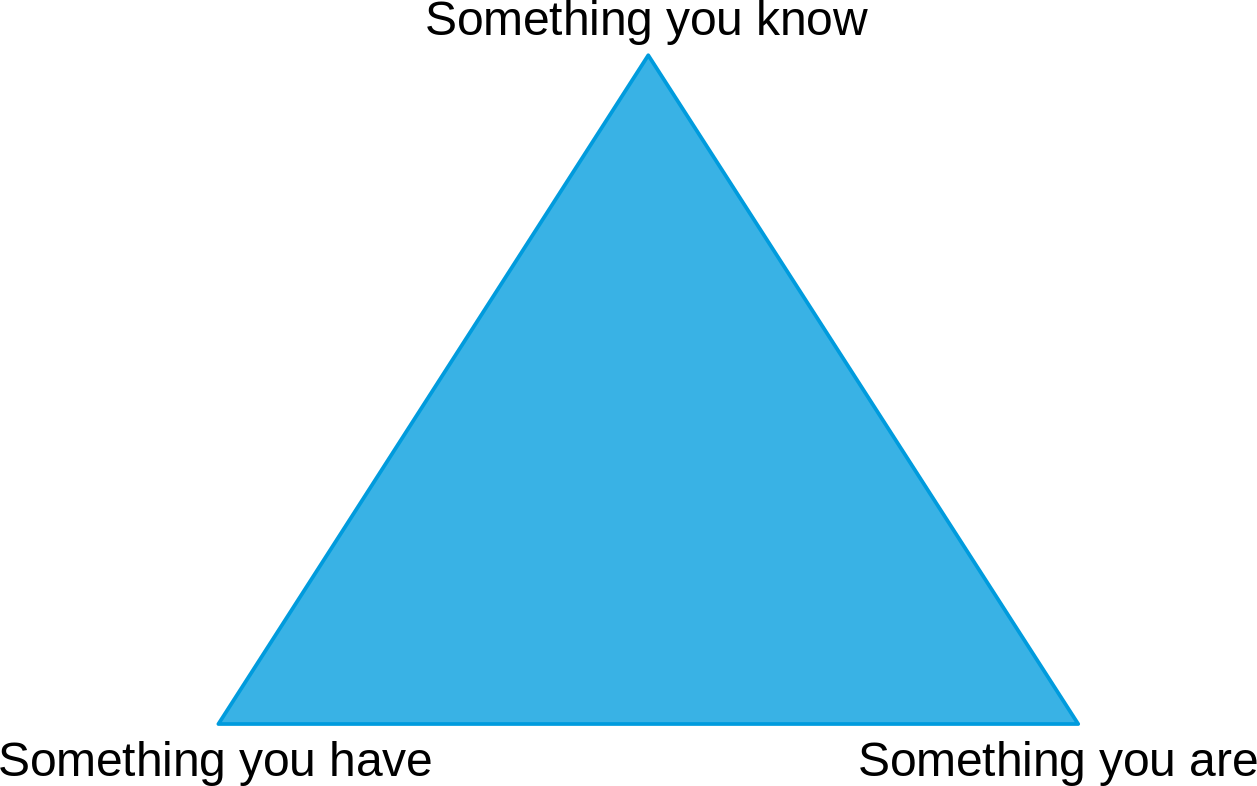
\includegraphics[width=\linewidth]{three-factors.png}
	\caption{The three factors of authentication. Something you know is information stored in your mind, something you have is an item in your physical posession, and something you are is a unique biometric property of your body.}
\end{figure}

In general, "something you know" is usually some text which you have memorized as a password. "Something you have" is usually a smartphone that can receive text messages or has an OTP (one-time password) app installed, a physical security key, or a smart card. "Something you are" is usually your fingerprint, iris pattern, face shape, or some other biometric information which is unique to you. As a whole, these are the three factors of authentication by which humans can identify themselves to a computing system. You may be familiar with the term "two-factor authentication", which refers to using two of these factors to authenticate someone. Two-factor authentication systems almost always use a combination of "something you know" along with either "something you have" or "something you are".

When authenticating to websites and applications, there are some scenarios which will likely always require a password. Most of these scenarios apply in a business or organizational context, but some do apply to personal usage. In some cases these authentication scenarios can be improved by adding a second factor to increase the security of an account, but it would not be feasible or desirable to remove the password.

\begin{itemize}
	\item Organizational person and non-person accounts
	\item Database accounts
	\item Windows, Mac, \& Linux local accounts
	\item Disk \& file encryption
	\item WiFi
	\item SSH (Secure Shell) keys
	\item PGP (Pretty Good Privacy) keys
	\item Crypto wallets
	\item Websites where SSO (Single Sign-On) integration is not desirable, such as banking sites
\end{itemize}

\section{Better Passwords}
Passwords today come in all shapes and sizes. Using a single password across all applications and websites would not only be insecure, but also infeasible. Creating a password for a new website often feels like a maniacal exercise with the various complexity requirements and limitations on length \& valid special characters. The recent web game "The Password Game" \autocite{passwordgame} represents this mental anguish quite well. These restrictions are usually due to inflexible code or database implementations on the website's backend, caused by the usage of legacy software or poor coding practices. However, there is a common set of requirements which exist for most general-purpose passwords - a lowercase letter, an uppercase letter, a number, and a special character. Given these common constraints, how should a strong passphrase be designed?

\begin{figure}[h]
	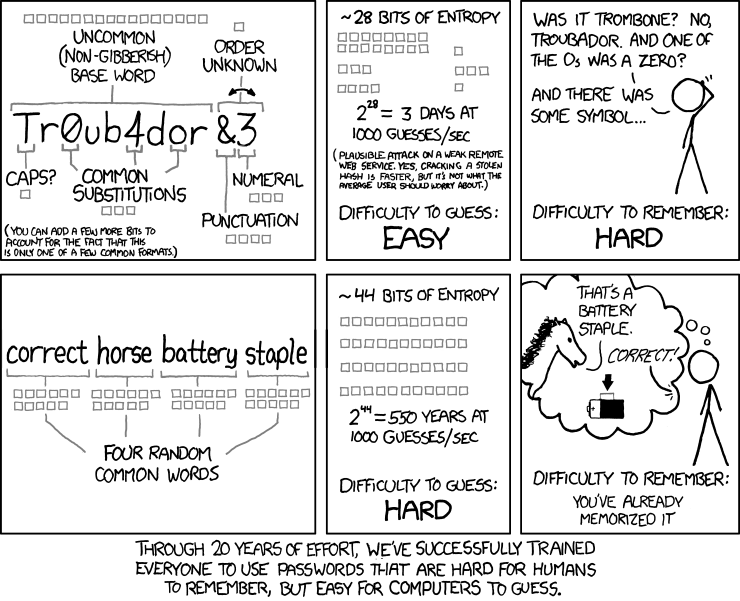
\includegraphics[width=\linewidth]{xkcd-936-password-strength.png}
	\caption{xkcd comic \#936. Source: Randall Munroe, \href{https://xkcd.com/936/}{https://xkcd.com/936/}.}
\end{figure}

If you've followed the online comic xkcd or pop culture references to passwords, you may have seen the comic above. It makes the case that a passphrase is much more desirable than a password for both memorability \& security. The terminology can be confusing here because a passphrase is essentially a type of password, but traditionally passwords are thought of as single words with some numbers or special characters added in. Thus when it is stated that a passphrase is better than a password, this is the type of password being referred to. The comic makes an excellent point about memorability, because remembering a semi-random string of letters, numbers, and special characters mixed together is not an easy task. It's also much easier to type a password into a computer when reading it from another device if the password parts can be grouped into larger items instead of individual characters.

It's unclear what word list the xkcd comic is referencing in its calculation of \textasciitilde44 bits of entropy for the listed passphrase. Password entropy is a measure of the strength of a password, which is calculated as the number of possible passwords which could have been generated when a password was chosen. This represents the worst-case scenario for you where someone who is trying to guess your password knows how you generated it. Bits of entropy is used as a measurement to make differing password strengths easier to compare. If you randomly choose 4 words for a passphrase and you can reliably recall 1,000 words from memory, then there are 1,000\textsuperscript{4} possible passwords which could be generated in this scenario. Taking the log base 2 of this number shows that this password has \textasciitilde40 bits of entropy.

The Electronic Frontier Foundation (EFF) has published a method for generating secure passphrases called "EFF Dice-Generated Passphrases" \autocite{effdice} which uses a similar approach to the xkcd comic. This is derived from a method of generating passphrases called Diceware \autocite{diceware}, which uses a numbered list of words and rolls of physical dice to generate a passphrase. Both methods use a word list with 7,776 words by default, and the EFF method recommends using 6 words. Diceware recommends using at least 5 words. A passphrase generated by the EFF method might look like this:
\\~\\
\centerline{willfully abridge cleat pending mascot squiggly}
\\~\\
This is a strong passphrase and has \textasciitilde78 bits of entropy:
\begin{align*}
& 7,776\textsuperscript{6} = \textasciitilde2.21 * 10\textsuperscript{23} \\
& log\textsubscript{2}(7,776\textsuperscript{6}) = \textasciitilde78
\end{align*}
If an attacker attempted to guess this passphrase via brute-force at a rate of 1,000 passphrases per second, it would take approximately 3.5 trillion years on average to guess it correctly. This is fairly secure, even against an attacker utilizing a GPU for password hash cracking. A more detailed analysis of the strength will appear later in this paper. There is one usability caveat though, and that is that a passphrase like this does not satisfy the most common constraints for passwords. It can only be used in scenarios where there is no password policy or a very unrestrictive password policy which allows someone to use only lowercase alphabetic characters. The vast majority of websites and organizations will not accept such a password. Can a method be created that is equally as strong and more usable?

% CREATION (creating the passphraser format)
\section{A New Algorithm}
A new passphrase-generation algorithm can be implemented which does not have the same limitations as those previously mentioned. It needs to generate strong passphrases but still meet the common password policy requirements of at least one lowercase letter, uppercase letter, number, and special character. The passphrases it generates also need to be memorable. The capability of human memory varies from person to person, but there are some well-defined general limits. Research in human psychology indicates that humans can generally repeat back around seven items (i.e. digits, letters, or words) immediately after being shown them in a sequence \autocite{magicnumberseven}. More recent research shows that humans can can easily recall between three and five items from active memory \autocite{magicalmysteryfour}. In everyday life in the United States, pieces of data which are commonly remembered such as phone numbers, social security numbers, and full names usually have a sequence of three items. For the sake of making this new passphrase-generation algorithm as accessible as possible, the lower bound of three items is used to determine how many words should be included in the generated passphrase.

In addition to words, numbers and special characters need to be included. Substituting these into words makes recalling a word more difficult because this is not how the word appears in natural language. Instead, special characters and a number are sequentially inserted between the words in the passphrase. For the sake of consistency a generated passphrase will always begin with a number or a special character. This can also reduce the likelihood that the passphrase will be guessed efficiently via brute-force because passwords usually begin with an alphabetic character \autocite{mostcommonpasswords}. In summary, two special characters and a number are used in order to have three words and three non-words. The 32 special characters in the ASCII character set are used for simplicity. When considering the number, early research on this algorithm used two-digit numbers but this did not generate enough entropy in the final passphrase. As a result, a four-digit number is used. This can be thought of as a four-digit year in order to make it more memorable. The majority of calendar systems in the world use four-digit years and thus most humans are familiar with recalling a four-digit number as a year. Thinking of this number as a year also typically reduces the syllables required to recall it by removing the words "hundred" and "thousand" from the number's verbal description. The number 1015 can be remembered as "ten fifteen" instead of "one thousand and fifteen", and the number 1969 can be remembered as "nineteen sixty nine" instead of "one thousand nine hundred and sixty nine".

Lastly, the issue of uppercase versus lowercase letters needs to be considered. The first letter of each word in the passphrase could be capitalized, but instead one of the three words is entirely capitalized in order to provide three times more entropy. If \textit{w} represents a lowercase word and \textit{W} represents an uppercase word, then the generated passphrase can have three variations of word sequences: \textit{wwW}, \textit{wWw}, and \textit{Www}.

After choosing the formatting for each item in the generated passphrase, there are nine possible passphrase formats that can be generated using this new algorithm. \textit{w} represents a lowercase word, \textit{W} represents an uppercase word, \textit{n} represents a number, and \textit{s} represents a special character.

% [h] is used below to specify that the table should appear below the previous text
% https://stackoverflow.com/questions/1673942/latex-table-positioning
\begin{table}[h] % Single column table
	%\caption{}
	\centering
	\begin{tabular}{l|l|l}
		%\toprule
		\multicolumn{3}{c}{Passphrase Formats} \\
		%\cmidrule(r){1-3}
		\midrule
		s w s w n W & s w s W n w & s W s w n w \\
		s w n w s W & s w n W s w & s W n w s w \\
		n w s w s W & n w s W s w & n W s w s w \\
		\bottomrule
	\end{tabular}
	\label{tab:passphraseformats}
\end{table}

A passphrase generated by Passphraser will look like this:

\centerline{*password2023security-INCREASED}


% WORDLIST (description of the Passphraser wordlist)
\section{Word List}
The word list used for Passphraser needs to be very large in order to generate enough entropy in the final passphrase. Creating the word list was surprisingly one of the most challenging parts of this work. There are not many word lists of sufficient size available for free on the internet. And of those that are available, many contain items which are not actually English words. After a great deal of research, the GitHub repository dwyl/english-words was chosen as the initial source of the word list \autocite{dwylwordlist}. The file \textit{words\_alpha.txt} was referenced as it contains only words with letters and no numbers or symbols. This list contains 370,105 words at the time of writing. The initial Passphraser wordlist published on GitHub \autocite{passphraserwordlist} is a subset of this list, with three modifications.

The first modification was to remove words which are not found in US English dictionaries. This was done by programmatically comparing the word list with several dictionaries to filter out words which did not match. Words such as \textit{crazycat}, \textit{deregulationize}, and \textit{preoccupative} are examples of those which were removed.

The second modification was to remove words which are generally considered obscene or which are generally used to disrespect people based on their physical or mental attributes. Everyone should have a positive experience when using Passphraser, no matter who they are. Many website articles were helpful in determining which words should be removed, and it is expected that some others may be removed in the future as language evolves. Given the volume of US English words available, the impact of removing such words is negligible when analyzing the entropy of generated passphrases.

The third modification was to remove words which have less than five letters or more than nineteen letters. This is done to ensure a minimum and maximum length of the generated passphrase. If three five-letter words are chosen then the resulting passphrase will have 21 characters, and if three nineteen-letter words are chosen then the resulting passphrase will have 63 characters. The lower bound is implemented in order to ensure that all generated passphrases are at least 20 characters, and the upper bound is implemented to ensure that all generated passphrases can be used as a WiFi password, since WiFi itself has a maximum password length of 63 characters.

After performing these modifications, the initial Passphraser word list has 181,552 words. This is sufficient to generate a reasonable amount of entropy as will be shown in the next section. The list itself has been published on GitHub under a public domain license, which is the same license as the dwyl/english-words list. Anyone is free to use this word list for any purpose.

% ANALYSIS (mathematical analysis of the passphraser format)
\section{Analysis}

In order to determine the entropy of a passphrase generated by the Passphraser algorithm, the number of possible variants can be calculated. There are nine formats in total --- each with three words, two special characters, and one four-digit number. There are 181,552 possible words, 32 possible special characters, and 9000 possible four-digit numbers (1000 to 9999). The formula for calculating the passphrase entropy looks like this:

\begin{align*}
	& 9 * 181,552\textsuperscript{3} * 32\textsuperscript{2} * 9000 = \textasciitilde4.96 * 10\textsuperscript{23} \\
	& log\textsubscript{2}(9 * 181,552\textsuperscript{3} * 32\textsuperscript{2} * 9000) = \textasciitilde79
\end{align*}

The total number of possible passphrases for Passphraser is more than twice that of the EFF Dice 6-word algorithm previously discussed, and the two algorithms have almost the same entropy. This looks like a satisfying result, but to get a more familiar real-world understanding of the strength of this passphrase it can be compared to the strength of fully-random passwords comprised of any of the 26 lowercase letters, 26 uppercase letters, 10 digits, and the 32 ASCII special characters --- 94 possible characters in total.

\begin{table}[h] % Single column table
	\centering
	\begin{tabular}{l l l}
		\multicolumn{3}{c}{Password Strengths} \\
		\midrule
		& Combinations & Bit Entropy \\
		\cmidrule(l){2-3}
		Random 6-character & \textasciitilde6.90 * 10\textsuperscript{11} & \textasciitilde39 \\
		xkcd 4-word & \textasciitilde1.76 * 10\textsuperscript{13} & \textasciitilde44 \\
		Random 7-character & \textasciitilde6.48 * 10\textsuperscript{13} & \textasciitilde46 \\
		... & ... & ... \\
		Random 11-character & \textasciitilde5.06 * 10\textsuperscript{21} & \textasciitilde72 \\
		EFF Dice 6-word & \textasciitilde2.21 * 10\textsuperscript{23} & \textasciitilde78 \\
		Random 12-character & \textasciitilde4.76 * 10\textsuperscript{23} & \textasciitilde79 \\
		Passphraser & \textasciitilde4.96 * 10\textsuperscript{23} & \textasciitilde79 \\
		Random 13-character & \textasciitilde4.47 * 10\textsuperscript{25} & \textasciitilde85 \\
	\end{tabular}
	\label{tab:passwordstrengths}
\end{table}

In conclusion, a passphrase generated by Passphraser effectively has the same strength as a 12-character fully-random password. The ability to recover a password of this strength is very subjective depending on the capabilities of the individual or organization attempting to recover it from a password hash. A lone hacker with a single desktop GPU will have a much different recovery time than the United States National Security Agency (NSA). However, some well-known password length recommendations are a good indicator of reliable password strength. NIST Special Publication 800-63B, which is used to set digital identity standards for US government agencies, recommends an 8-character minimum length \autocite{nistpassword}. Microsoft also recommends a minimum of 8 characters for organizational accounts \autocite{microsoftpassword}, and Google recommends a minimum of 12 characters for personal accounts \autocite{googlepassword}. A password generated by Passphraser thus has sufficient strength for standard modern-day requirements.

One final consideration is that the entropy rating above indicates the strength of a Passphraser password in the worst-case situation, where an attacker knows that the password they are attempting to recover was generated by Passphraser. If this is not known then it would take much longer for the password to be recovered. This knowledge is dependent on the situation of the individual who created an account password with Passphraser and the individual attempting to recover the password.

% FUTURE WORK (valid website list, additional languages, etc.)
\section{Future Work}

Future efforts on Passsphraser may be dedicated to four areas. One goal is to publish a list of websites where Passphraser passwords can be effectively used. Nearly every website has varying password complexity \& length requirements, and it would be helpful to people using Passphraser to know whether it is safe to use for a specific website account without analyzing the website's password complexity requirements. Passphraser should only be considered safe to use for a website if every possible password generated by Passphraser could be used as a valid account password on that site.

A second goal for Passphraser is integration of its algorithm with password management applications. The code for Passphraser is published as a command-line application today and there are no plans to make a GUI version. Rather than reinventing the wheel, it would make sense to integrate with popular password managers which already have robust password generators.

A future area of research for Passphraser is the usability \& security of passphrases with an arbitrary number of words. The algorithm described in this paper uses three words, but it is possible to specify the number of words desired when running the Passphraser command-line application. Passphrases with an odd number of words \textit{W} have \textit{(W+1)/2} lowercase words \& special characters and \textit{(W-1)/2} uppercase words \& numbers. Passphrases with an even number of words \textit{W} have \textit{W/2} lowercase words, special characters, uppercase words, and numbers.

Another future area of research for Passphraser is the inclusion of additional languages for password generation. The feasibility of this primarily depends on the availability of word lists of sufficient size and the legality of obtaining \& publishing those word lists publicly online. During the creation of the Passphraser wordlist the author found that the laws regarding publishing a compiled list of words significantly varies by country. The details of the legal situation in the United States can be found on the Passphraser wordlist repository README on GitHub \autocite{passphraserwordlist}.

%----------------------------------------------------------------------------------------
%	 REFERENCES
%----------------------------------------------------------------------------------------

\printbibliography % Output the bibliography

%----------------------------------------------------------------------------------------

\end{document}
